\chapter{Background Theory of Bayesian Techniques and WEST Interferometry}

This chapter aims to equip the reader with necessary background theory required to reproduce this work and to understand the origin of the inferred electron density profiles presented in the results. It first describes a tokamak fusion device and some relevant physics concepts behind its function. It then describes in a high level manner the inference carried out by Blaise Faugeras and team with their code known as \gls{nice} \cite{nice}. After the chapter outlines Bayesian inference and it's connection with \gls{gpr}. Then the \gls{gpr} method is explained in detail for a simple regression problem. At this point Interferometry is introduced in enough detail that the \gls{gpr} method can be altered to infer the electron density profile. The key factor being the new responce matrix. There are various options for advanced alterations that are then explained here and explored in the results section.

\begin{figure}
  \centering
  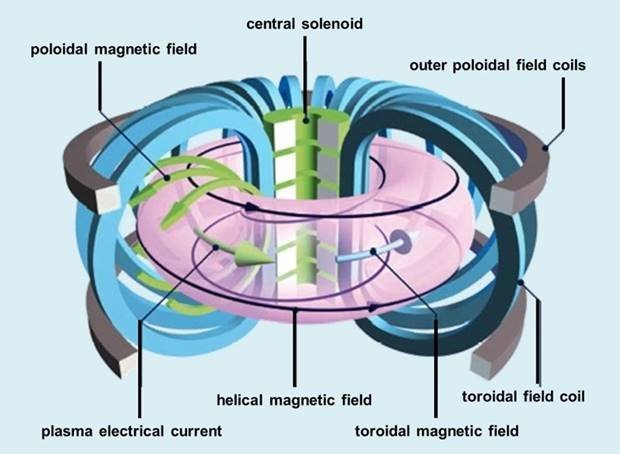
\includegraphics[width=10cm]{images/tokamak.jpg}
  \caption{Diagram of a tokamak and relevant magnetic fields that create the helical particle trajectory \cite{tokamakSchema}.}
  \label{fig:tokamakSchema}
\end{figure}

Tokamak is a class of fusion device whose name comes from the abbreviation of a Russian phrase which means "toroidal chamber with magnetic coils". It consists of a doughnut shaped vacuum chamber surrounded by powerful magnets that aim to confine a high temperature plasma that would otherwise vaporise the chamber. The plasma pressure and temperature are fundamental parameters in the context of nuclear fusion because they dictate the conditions required to overcome the electrostatic repulsion between positively charged atomic nuclei and bring them close enough for the strong nuclear force to initiate fusion reactions. In the core of stars like our Sun, the immense pressure and temperature generated by the gravitational collapse create the conditions where hydrogen nuclei (protons) can overcome their natural repulsion and fuse into helium, releasing a tremendous amount of energy in the process. To initiate fusion, hydrogen must be heated to temperatures in the range of tens of millions of degrees Celsius. In a tokamak, this is mainly accomplished with ohmic heating via a driving plasma current and neutral gas injection. This involves accelerating hydrogen ions to high speeds with electric fields and neutralising them the instant before they enter the chamber. The resulting plasma attains the required temperature, allowing nuclei to collide with sufficient energy for fusion reactions to occur. Figure \ref{fig:tokamakSchema} shows the position of various magnetic field coils within the tokamak. The toroidal magnetic field exerts an inward force on the plasma thus raising its pressure. A high pressure is required to increase the frequency of collisions so that the energy output could exceed the large heating energy input. The central solenoid induces a current in the plasma which produces the majority of the poloidal magnetic field. This field is essential for confinement but it also plays a key role in plasma stability. The outer poloidal field coils can be controlled in real time to help mitigate instabilities. A real time inference of the electron density profile would assist in identifying instabilities and informing the algorithm that drives the control coils to mitigate them. In addition to high temperature and pressure, the tokamak design seeks to maximize the confinement time of the plasma. This is essential to allow a sufficient number of fusion reactions to occur before the plasma cools down or loses its stability. The magnetic fields in a tokamak are carefully optimized to prevent rapid plasma loss and minimize heat loss through various mechanisms, including turbulent transport. The shape of the density profile has a large effect on the confinement time.

The combination of the toroidal and poloidal fields shown in figure \ref{fig:tokamakSchema} create a helical magnetic field within the plasma. Electrons and ions are accelerated in opposite toroidal directions by the central solenoid yet the both follow a trajectory along the magnetic field lines. This is because a charged particle moving across a magnetic field is succumb to a force perpendicular to its motion. This causes them to gyrate around the magnetic field lines and confines them to follow the magnetic field lines. This is an over simplification although a detailed description of particle motion within a magnetic field is not needed for the purpose of this thesis. It is enough to know that if a single charged particle was within a tokamak then it would perfectly follow a trajectory along the helical path of the magnetic field lines with a small gyration around the field line. When many particles are introduced then collisions can interrupt these trajectories, yet in many models used for data analysis the assumption that particles follow the magnetic field lines is used, including within this thesis. 

The magnetic field lines are confined to magnetic flux surfaces, figure \ref{fig:magfluxsurf}. The toroidal and poloidal flux is constant on magnetic flux surfaces, there is 0 flux across magnetic flux surfaces. Since we assume that the particles follow the magnetic field lines which are strictly bound to these surfaces, we also assume that the density is constant on these surfaces. This allows the density of the entire cross-section to be expressed with a 1D profile as a function of normalised radius $\rho$, figure \ref{fig:nice_example}. Where $\rho$ is 0 at the plasma core and 1 at the edge. At the core the poloial magnetic flux is 0 and the edge is the last closed flux surface. Particles past the edge are no longer bound and may interact with the plasma wall. The existance of nested magnetic flux surfaces shown in figure \ref{fig:magfluxsurf} rely on the ideal \gls{mhd} assumptions. Experiments frequently discover magnetic islands which discredits the assumption of nested flux surfaces. The electron density profiles infered rely on this assumption although for many applications, such as real time control a highly accurate infernce is often not required.

\begin{figure}
  \centering
  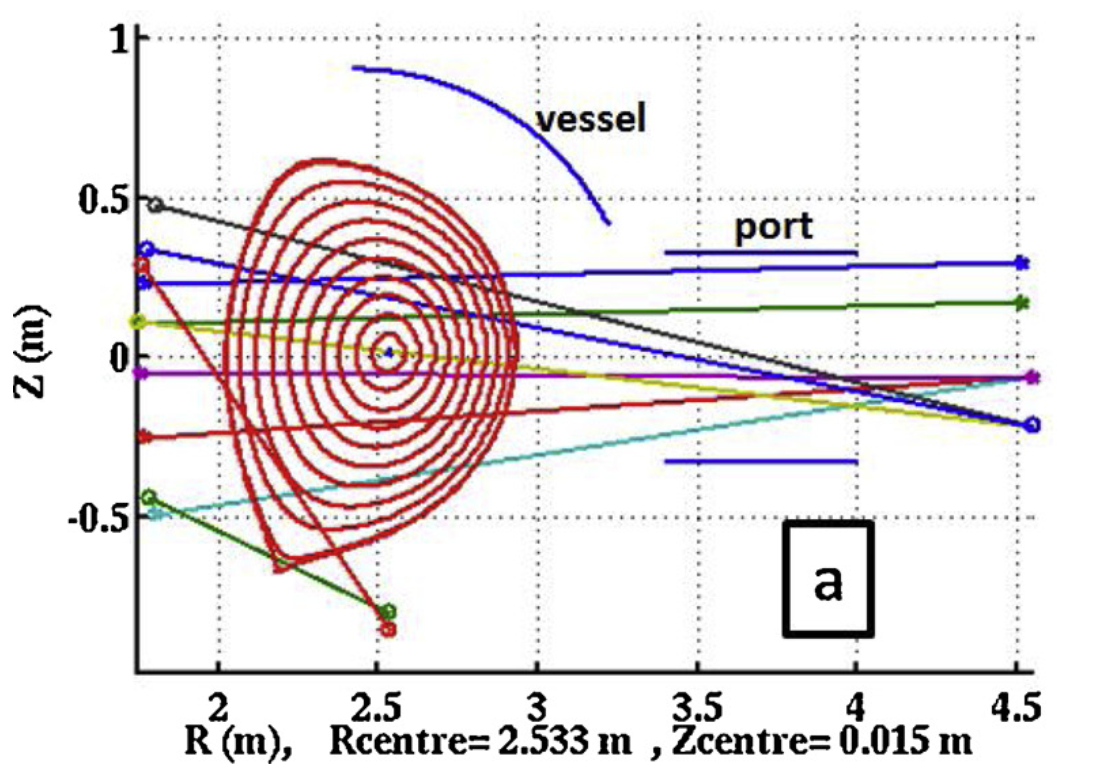
\includegraphics[width=10cm]{images/magfluxsurf.png}
  \caption{The magnetic flux surfaces and interfero-polarimetry laser geometry for a cross-section of the WEST tokamak \cite{reneintpol}.}
  \label{fig:magfluxsurf}
\end{figure}

\gls{nice} is an equilibrium reconstruction code developed for the WEST tokamak. It is relevant because it computes an inference of the electron density profile that is available for comparison to the profile inferred in this work, although \glspl{nice} main objective is to infer the shape and position of the magnetic flux surfaces. \gls{nice} uses magnetic diagnostics and at WEST these include 421 pickup coils, 36 flux loops and 12 Rogowski coils \cite{westmagdiag}. The magnetic diagnostics provide the majority of the information. \gls{nice} also uses interferometry, polarimetry, motional stark effect and pressure measurements. Section \ref{} explains how interferometry and polarimetry together can provide information about the poloidal magnetic field, which directly affects the magnetic flux and thus magnetic flux surfaces. \gls{nice} performs the inference by minimising a cost function. The cost function determines how well a physical state of the system matches the data received. A state being a specific position and shape of the magnetic flux surfaces and electron density profile. This requires a forward model. The forward model takes a state of the system attempts to compute the signals that would be received by error free diagnostics, if that state was the ground truth. The forward model is a simplified mathematical representation of the measurement process and can never be 100\% accurate. This introduces errors into the inference that need to be accounted for. The signals from the forward model can be compared to the actual signals received by the diagnostics in order to compute the cost function. By minimising the cost function the state that best matches the data is found. \gls{nice} uses \gls{sqp} as the minimisation algorithm. The optimal state of the system is then stored in the \gls{imas} database for WEST. This includes the 1D electron density profile used as a comparison for the profile inferred in this work using \gls{gpr}. \gls{nice} also imposes regularisation terms on their cost function. These penalise the cost function when state properties have features that disagree with prior knowledge. This includes smoothness. We expect the magnetic flux surfaces and electron density profile, to be continuous and smooth. A state inputted into the cost function that is not smooth triggers the regularisation term which causes the cost function to be larger. Minimising the cost function now also leads to smooth magnetic flux surfaces and electron density profile. This leads into a difficult question, how smooth should it be? They also have a regularisation term to penalise the cost function if the electron density profile is far from 0 at the last closed flux surface or plasma edge. It is prior knowledge that the electron density is near 0 at the plasma edge. How close to 0, and how strong should the regularisation be is still an open question. This work's \gls{gpr} approach has  direct analogs to these regularisation terms, section \ref{}. Figure \ref{fig:nice_example} shows an example of a \gls{nice} inferred electron density profile. It is modeled with a cubic spline function. It is the parameters of the cubic spline that are inputted into the cost function. The errors are calculated using a sensitivity method. In short the error is deemed larger for the electron density of a particular normalised radius if a large change in the density leads to a small change in the cost function. In this case we cannot be certain what density is more true because many lead to a similarly low cost function and thus match the data similarly well. To include some more details, the \gls{sqp} minimisation algorithm computes the hessian of the cost function for minimisation, but this hessian can also be used to measure the sensitivity and thus the errors. The diagonal of the hessian contains the second differential of the cost function for each input parameter. This describes the curvature of the cost function in the direction of each parameter. A smaller curvature means a smaller sensitivity and thus a larger error.

\begin{figure}
  \centering
  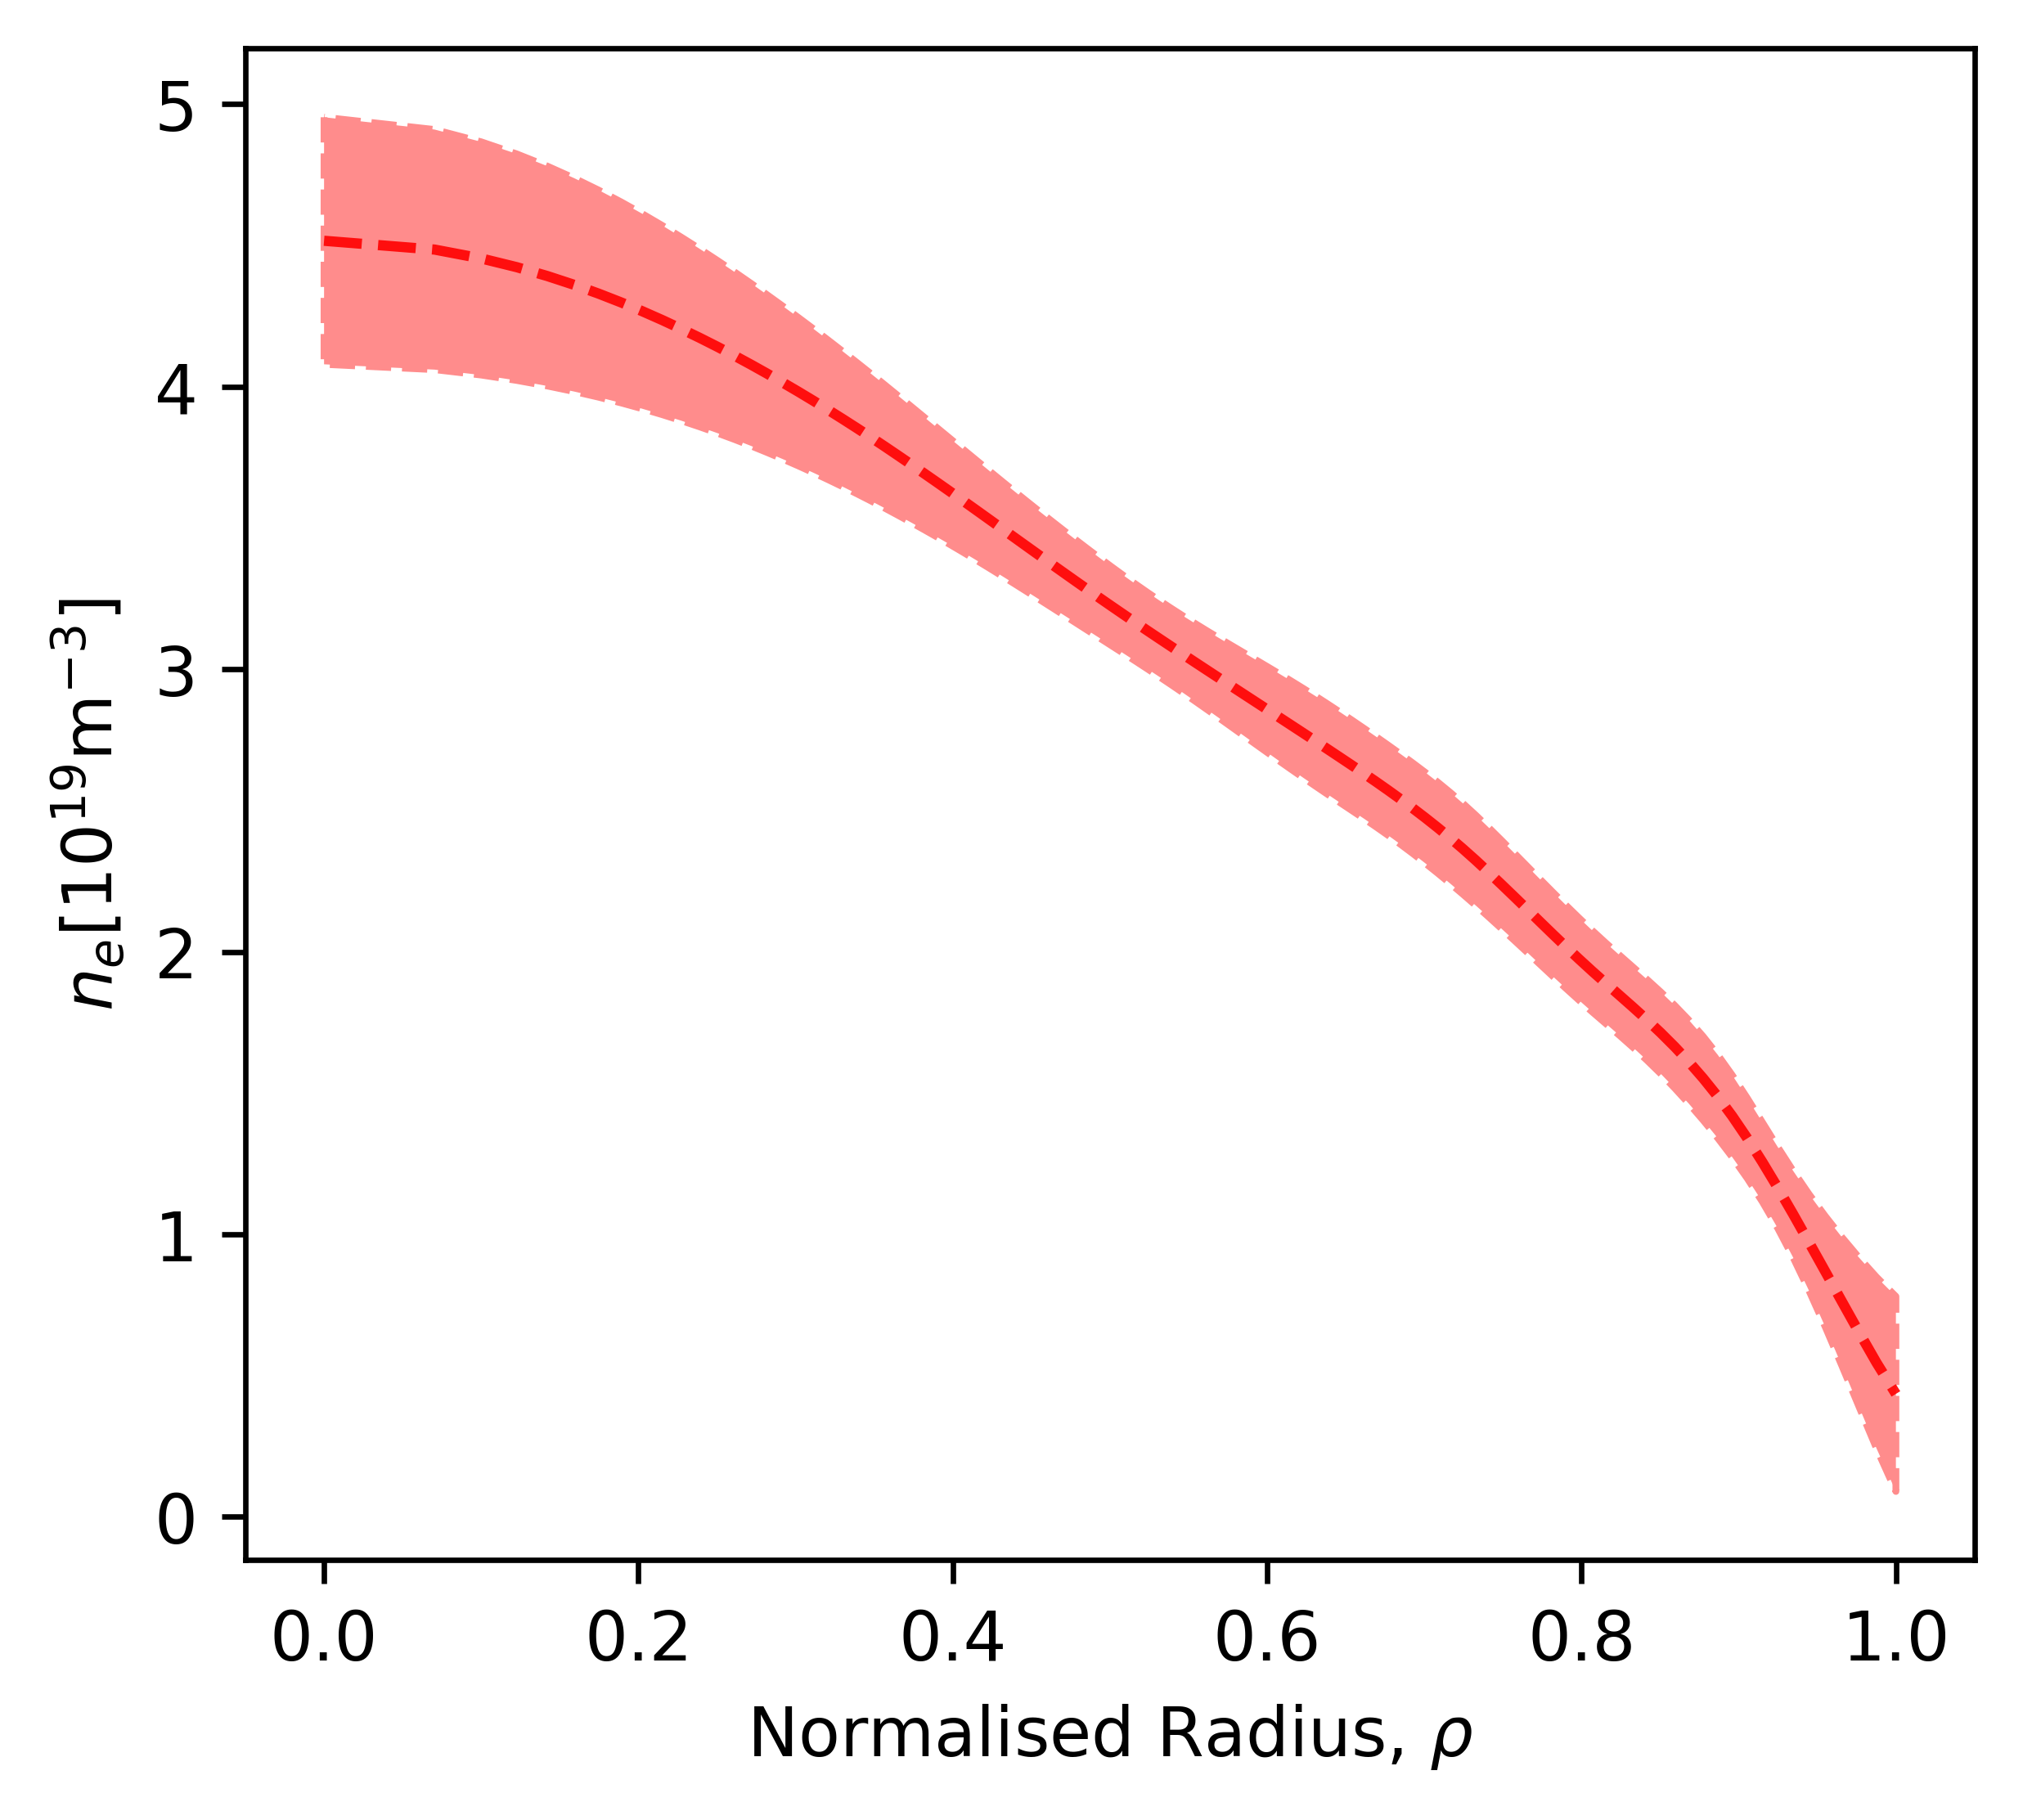
\includegraphics[width=10cm]{images/niceExample.png}
  \caption{Electron density profile inferred by \gls{nice} for an instance in time within the \gls{west} tokamak.}
  \label{fig:nice_example}
\end{figure}

This work aims to use Bayesian inference to obtain the electron density profile. Bayes theorem is written in equation \ref{eq:bayesth} for a physical quantity of interest $q$. The posterior $P(q|D,I)$ is the probability density distribution of $q$ given the measured data $D$ and some prior information $I$. The maximum of the posterior is the most probable value of $q$ given the data and prior information. The uncertainty of $q$ can also be obtained from the posterior, in this work the posterior will be Gaussian and so the error is simply the standard deviation. The likelihood $P(D|q,I)$ is the probability density function that expresses the probability of the measured data given a fixed value of $q$ and the prior information. The likelihood is described by the experimental error for the data collection. The prior $P(q|I)$ contains information assumed about $q$ before the data is taken. The marginal likelihood or evidence $P(D|I)$ is simply the probability of the data given the prior information only. For posterior computation the marginal likelihood serves as a normalisation factor. Normalisation is often carried out with other means to simplify the posterior computation. Although the marginal likelihood can be used to tune the prior. Sometimes the degree or strength of prior information is uncertain and by finding the strength that maximises the marginal likelihood we find the prior that match's the data the best. Maximising the marginal likelihood to tune the prior also aids to avoid over-fitting the posterior as the trade off between model complexity and data-fit is automatic via the Occam's razor principle \cite{oscraz}. The marginal likelihood method is powerful although it is important to remember that it is not perfect and does not guarantee the most accurate posterior.

\begin{equation} 
    P(q|D,I) = \frac{P(D|q,I) P(q|I)}{P(D|I)}
    \label{eq:bayesth}
\end{equation}

\gls{gpr} is a form of Bayesian inference where we assume these distributions can be expressed with multivariate Gaussian distributions. When the prior and posterior have the same form then the prior is known as a conjugate prior. This simplifies the inference as it is possible to find a closed form expression of the posterior. Without a closed form expression the posterior must be approximated with sampling techniques. \gls{gpr} is the technique used in this work to infer the electron density profile from interferometry data. First the technique is introduced for a simple regression problem where we wish to fit a curve to a set of points. 

\begin{equation}
\mathcal{N}(Y, \Vec{\mu}, \overline{\overline{\Sigma}}) = \frac{1}{\sqrt{4\pi^2|\overline{\overline{\Sigma}}|}} e^{{-\frac{1}{2}(\Vec{y}-\Vec{\mu})^T\overline{\overline{\Sigma}}^{-1}(\Vec{y}-\Vec{\mu})}}
\label{eq:mvg}
\end{equation}

The multivariate Gaussian expression \ref{eq:mvg} can be used to model a curve and its uncertainty, as illustrated in the violin plot \ref{fig:mvg}. The mean vector $\Vec{\mu}$ holds the $y$ values of the curve at regular intervals along the $x$ axis. The diagonal of the covariance matrix holds the standard deviations of each Gaussian of the multivariate which represents the errors of the curve. Figure \ref{fig:mvg} has 10 Gaussians but in practice many are used to ensure a smooth curve. This will be used to represent the result of \gls{gpr} which is the most likely curve given the data. The uncertainty of this curve is represented by the standard deviation of the many Gaussians that make it up.  

\begin{figure}
  \centering
  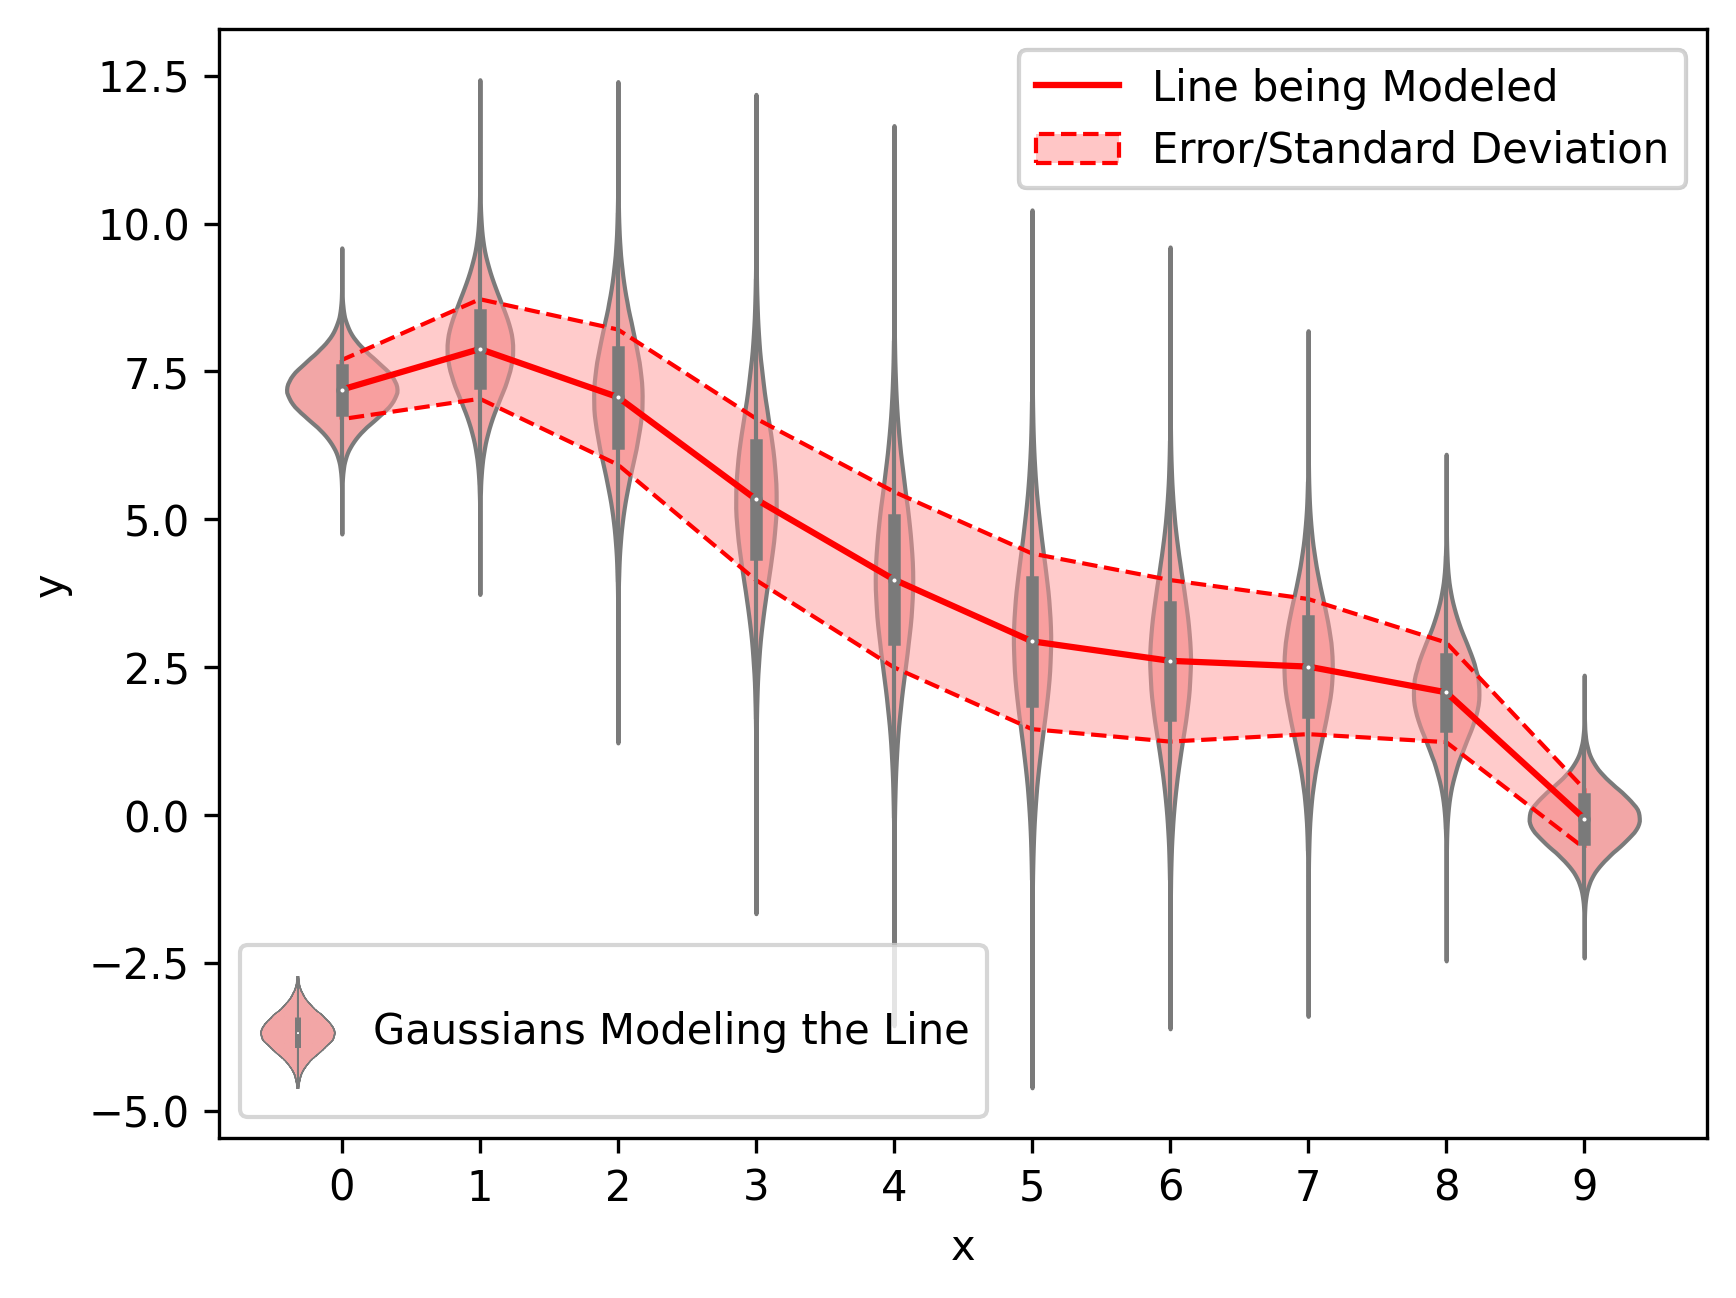
\includegraphics[width=10cm]{images/mvg.png}
  \caption{Illustrating how many Gaussians can model a line and its uncertainty.}
  \label{fig:mvg}
\end{figure}

The simple regression problem consists of points to which one would like to fit a smooth curve. To solve this using \gls{gpr} one must define their likelihood (equation \ref{eq:likelihood}) and prior (equation \ref{eq:prior}) as multivariate Gaussians. The many gaussians that make up these multivariate gaussians are visualised in \ref{fig:gprvis}. This visualisation method is perfect for the likelihood where the covariance matrix is diagonal. The multiple gaussians that make up the likelihood are not dependant on eachother and so representing them individually provides all the infomation in the likelihood. The prior has a more complex covariance matrix $\overline{\overline{K}}$, and figure \ref{fig:gprvis} does not have a complete representation of the priors form. In this simple implimentation the covariance between the prior's Gaussians can be completly encapsulated by a single number known as the lengthscale $l$ in equation \ref{eq:prior}. These visualisations of the varius distributions are helpful but to compute the posterior in figure \ref{fig:gprvis} one must understand the components of equations \ref{eq:posterior}, \ref{eq:likelihood}, \ref{eq:prior}, and how they can be combined to form the closed form equations \ref{eq:closedform}. In the posterior equation \ref{eq:posterior}, $\Vec{y}$ contains the random variables $y_i$ for regularly spaced positions $x_i$. Given the data the most probable values of these random variables is expressed in $\Vec{\mu}$ and their uncertinites in the diagonal of $\overline{\overline{\Sigma_{post}}}$. In the likelihood equation \ref{eq:likelihood} $\Vec{D}$, is a vector containing all the data/$y$-values from measurements at various $x$ positions. $\overline{\overline{R}}$ is known as the responce matrix and ensures that the mean vector of the multivariate gaussian $\overline{\overline{R}}\Vec{y}$ only contains values of $\Vec(y)$ at the same $x$ positions the data was recorded at. $\overline{\overline{R}}$ is essentially a filter that removes irrelevant $y_i$ values from $\Vec{y}$ for the mean vector of the likelyhood. In the likelihood of figure \ref{fig:gprvis} you can see an example of a given $\Vec{y}$ and the mean of each gaussian is the value on that line at the same $x$ position as the data point. $\epsilon$ is the experimental error of the measurements in $\Vec{D}$. In the prior equation \ref{eq:prior}, there are as many gaussians as in the posterior but each of these gaussians have a mean of 0. The $\Vec{0}$ symbol represents a vector of zeros the same length as the vector $\Vec{y}$ of random variables. To aid visualisation the prior in figure $\ref{fig:gprvis}$ only shows 5 out of the 101 gaussians used. The covariance matrix $\overline{\overline{K}}$ is constructed using the kernel $K_{ij}$. The main role of the amplitude ($\sigma$) in the kernel is to set the prior strength. The length scale ($l$) sets the strength of corelation of neighbouring gaussians. A low length scale that is small relative to the size of the curves features along $x$ means that only gaussians close in $x$ are highly correlated. Gaussians far have a low correlation meaning they can have a very different mean value. A low length scale allows the fitted curve to have more complexity simililar to a high order polynomial and can lead to overfitting. A high length scale limits the fits ability to curve sharply leading to a simple model similar to a low order polynolial, leading to underfitting. A very high length scale leads to an almost linear fit, every time. This prior is far from perfect. For instance it is often known that the infered values must be positive, for example you cannot have a negative electron density. Since the prior mean vector is set to $\Vec{0}$ a negative value is as likely to be infered as a positive value. Since it is gaussian values close to 0 are more likely to be infered than values far from 0. To mitigate this, high amplitude value can be used to lower the prior strength and allow the data in the likelyhod to have more influence on the posterior result. The kernel $K_{ij}$ in equation \ref{eq:prior} is known as the static exponential square kernel. It is a very commonly used kernel in \gls{gpr} but far from the only choice. The single value of length scale prevents the inference from haveing long smooth regions with few features followd by regions of high variability. This can be an issue when infering H-mode tokamak plasmas that have a sharp drop off in density at the edge. For these situations a non static kernel can be used that alows the lengthscale to be a function of $x$ which can then allow for posteriors of varying complexity. Regardless of the kernel used, deciding the optimal values of its parameters for a problem is not obvious. A common solution is to use the marginal likelyhood of equation \ref{eq:bayesth} as a loss function. The parameters that maxemise it can be found with gradient based methods. The marginal likelihood expresses the probability of the data and so maximising it finds the parameters that maxemises to probability of the data being measured. Although the marginal likelyhood method is also known for automatically deploying Occam's razor principle which finds a balance between closely fitting the data and having a simple model that accounts for the data's errors to have a more accurate inference \cite{oscraz} \cite{gp4ml}. Essentially maxemising the marginal likelihood avoids overfitting. Although this method is powerful it does not guarentee to produce parameters that lead to the most accurate fit. To get a more acurate fit, bayesian sampleing techniques can be used, although this is more computationally expensive. 

\begin{equation}
  \mathcal{N}(\Vec{y}, \Vec{\mu_{post}}, \overline{\overline{\Sigma_{post}}})
  \label{eq:posterior}
\end{equation}

\begin{equation}
  closed form
  \label{eq:closedform}
\end{equation}

\begin{equation}
    \mathcal{N}(\Vec{D}, \overline{\overline{R}}\Vec{y}, \overline{\overline{\Sigma_{li}}}),\hspace{0.5cm} \overline{\overline{\Sigma_{li}}} = 
      \begin{vmatrix}
          \epsilon & 0 & 0\\
          0 & \epsilon & 0\\
          0 & 0 & \epsilon
      \end{vmatrix}
    \label{eq:likelihood}
\end{equation}

\begin{equation}
  \mathcal{N}(\Vec{y}, \Vec{0}, \overline{\overline{K}}),\hspace{0.5cm} K_{ij} = \sigma e^{\frac{y_i - y_j}{2l^2}}
  \label{eq:prior}
\end{equation}

\begin{figure}
  \centering
  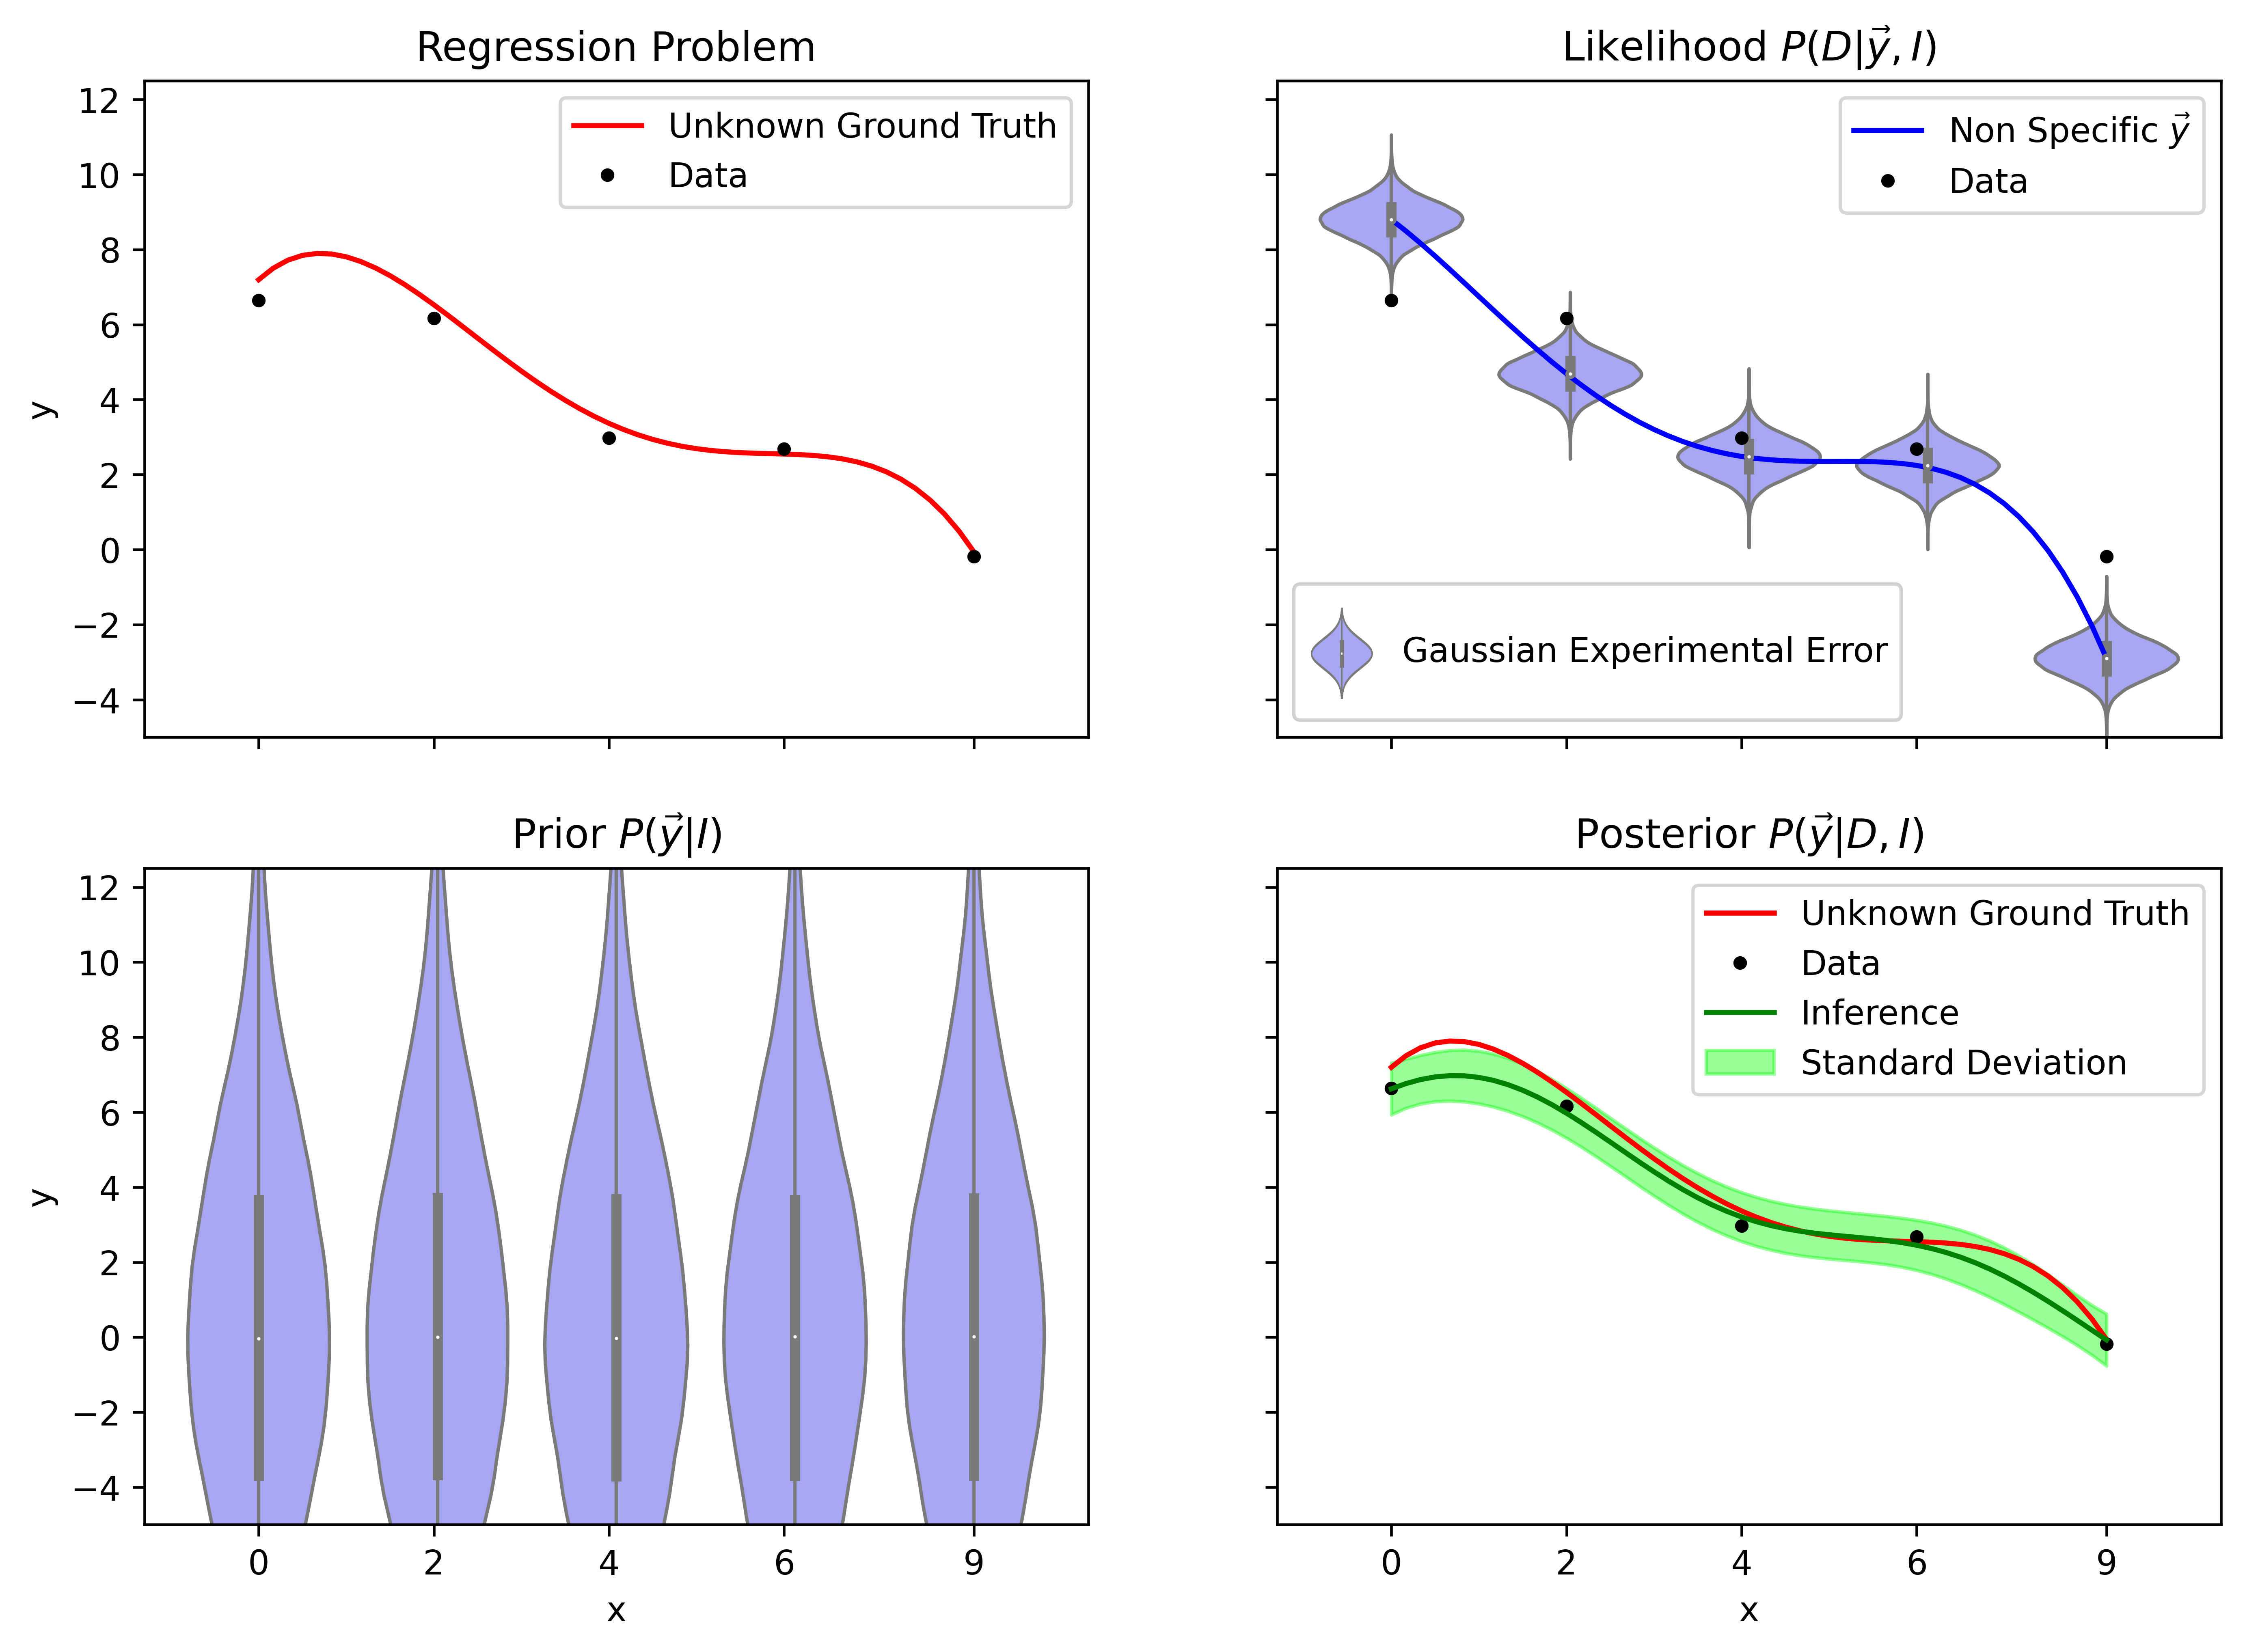
\includegraphics[width=10cm]{images/gprvis.png}
  \caption{A visualisation of the simple \gls{gpr} process. In truth the prior in this implementation has 101 Gaussians. Only five are shown to aid visualisation. The likelihood truly has the same number of Gaussians as the number of data points. The posterior has 101 Gaussians, their mean is shown by the green line, the standard deviation by the green shade, it is analogous to figure fig:mvg without the Gaussians full form being shown.}
  \label{fig:gprvis}
\end{figure}

%write about interferometry
Interferometry and polarimetry are two diagnostics obtained from the same hardware. Lasers are fired through the plasma at multiple angles. 

The geometry at \gls{west} is shown in figure 

\ref{fig:magfluxsurf}. The refractive index of the plasma is dependant on the electron density. The lasers slow and the phase shift can be measured. This phase shift is proportinal the line integrated electron density $\n_e$, along the line of sight of the lasers, equation \ref{eq:int_phase}, \cite{princPlasDiag}. The laser wavelength $\lambda$, is comnined with other common physical constants to assertain the constant of proportionality. For this reason WEST have stored the line integreated electron density as raw data in the IMAS database. This is the data that will be used for this work.

\begin{equation} 
  \label{eq:int_phase}
  \Delta\phi = \frac{\lambda e^{2}}{4 \pi \epsilon_0 m_e c^2 } \int n_e dl
\end{equation}

Polarimetry measures the faraday rotation angle of the lasers. The linearly polarised lasers experience a rotation as the circularly polarised components travel through the plasma at different speeds. This is due to the small gyration of the electrons around the margnetic field. The faraday rotation angle is proportinal to the line integrated density of $n_e B_{||}$ along the line of sight of the lasers. Where $B_{||}$ is the magnetic field strenghth paralell to the line of sight. Polarimetry has information about the electron density and this work could be extended to bcome a bayesian integrated analysis which includes this infomation in the inference. Currently only interferometry information is used. 

\begin{equation}
	\theta_F = \frac{\lambda^2 e^3}{8 \pi^2 c^3 \epsilon_0 m_e^2} \int n_e B_{||}dl
\end{equation}

To infer the electron density profile with interferometry information of an instant in time the \gls{gpr} process is alterd. $\Vec{y}$ becomes $\Vec{n_e}$ and the likelihood changes. The $\Vec{0}$ prior mean can remain the same, the amplitude $\sig$ and length-scale $l$ can also be optimised my maximising the marginal likelihood. The data is now in a different space and thus is the likelyhood. The responce matrix $R$ must be created so that it will transform a profile $\Vec{n_e}$ into what would be measured by an error free version of the \gls{west} interferometry system given $\Vec{\n_e}$ is the true profile. The result of $\overline{\overline{R}} \Vec{n_e}$ is a vector the same length as the data $\Vec{d}$ where each element corresponds to a different interferometry laser or channel. 

The responce matrix computation can be summarised in a few steps. \Gls{nice} provides the magnetic flux at a set of grid points on the tokamak cross section. It also provides the flux at a set of flux surfaces of known normalised radius $\rho$. A simple 1D interpolation can be used to determine the normalised radius at each grid point. Then using $\Vec{n_e}$ another 1D interpolation can be done to determine the electron density at each grid point. After the density at any point along a lasers line of sight can be computed using tringuar mesh interpolation. The line integrated density can be approximated as a sum of many electron densities points along the line of sight times the width of their seperation. The contribution of each point on the grid is a sum of all the mesh interpolation coefficiants used on that point. Each point can be associated to its nearest of 101 flux surfaces equally spaced in $\rho$. This way the contribution of each flux surface is a sum of the contribution at each of its associated grid points. These contributions are placed in a vector for that line of sight. Each line of sight has its own flux surface contribution vector. When these are placed as rows in a matrix we have the responce matrix.




To summarise the electron density profile is important as it plays a key role in determining the energy confinement time and informing real time control systems. With the assumption of magnetic flux surfaces one can express it as a 1D profile, \ref{fig:nice_example}. \gls{nice} is an equilibrium re-construction code that also infers the electron density profile that can be used as a comparison in this thesis. 

% \begin{figure}
%   \centering
%   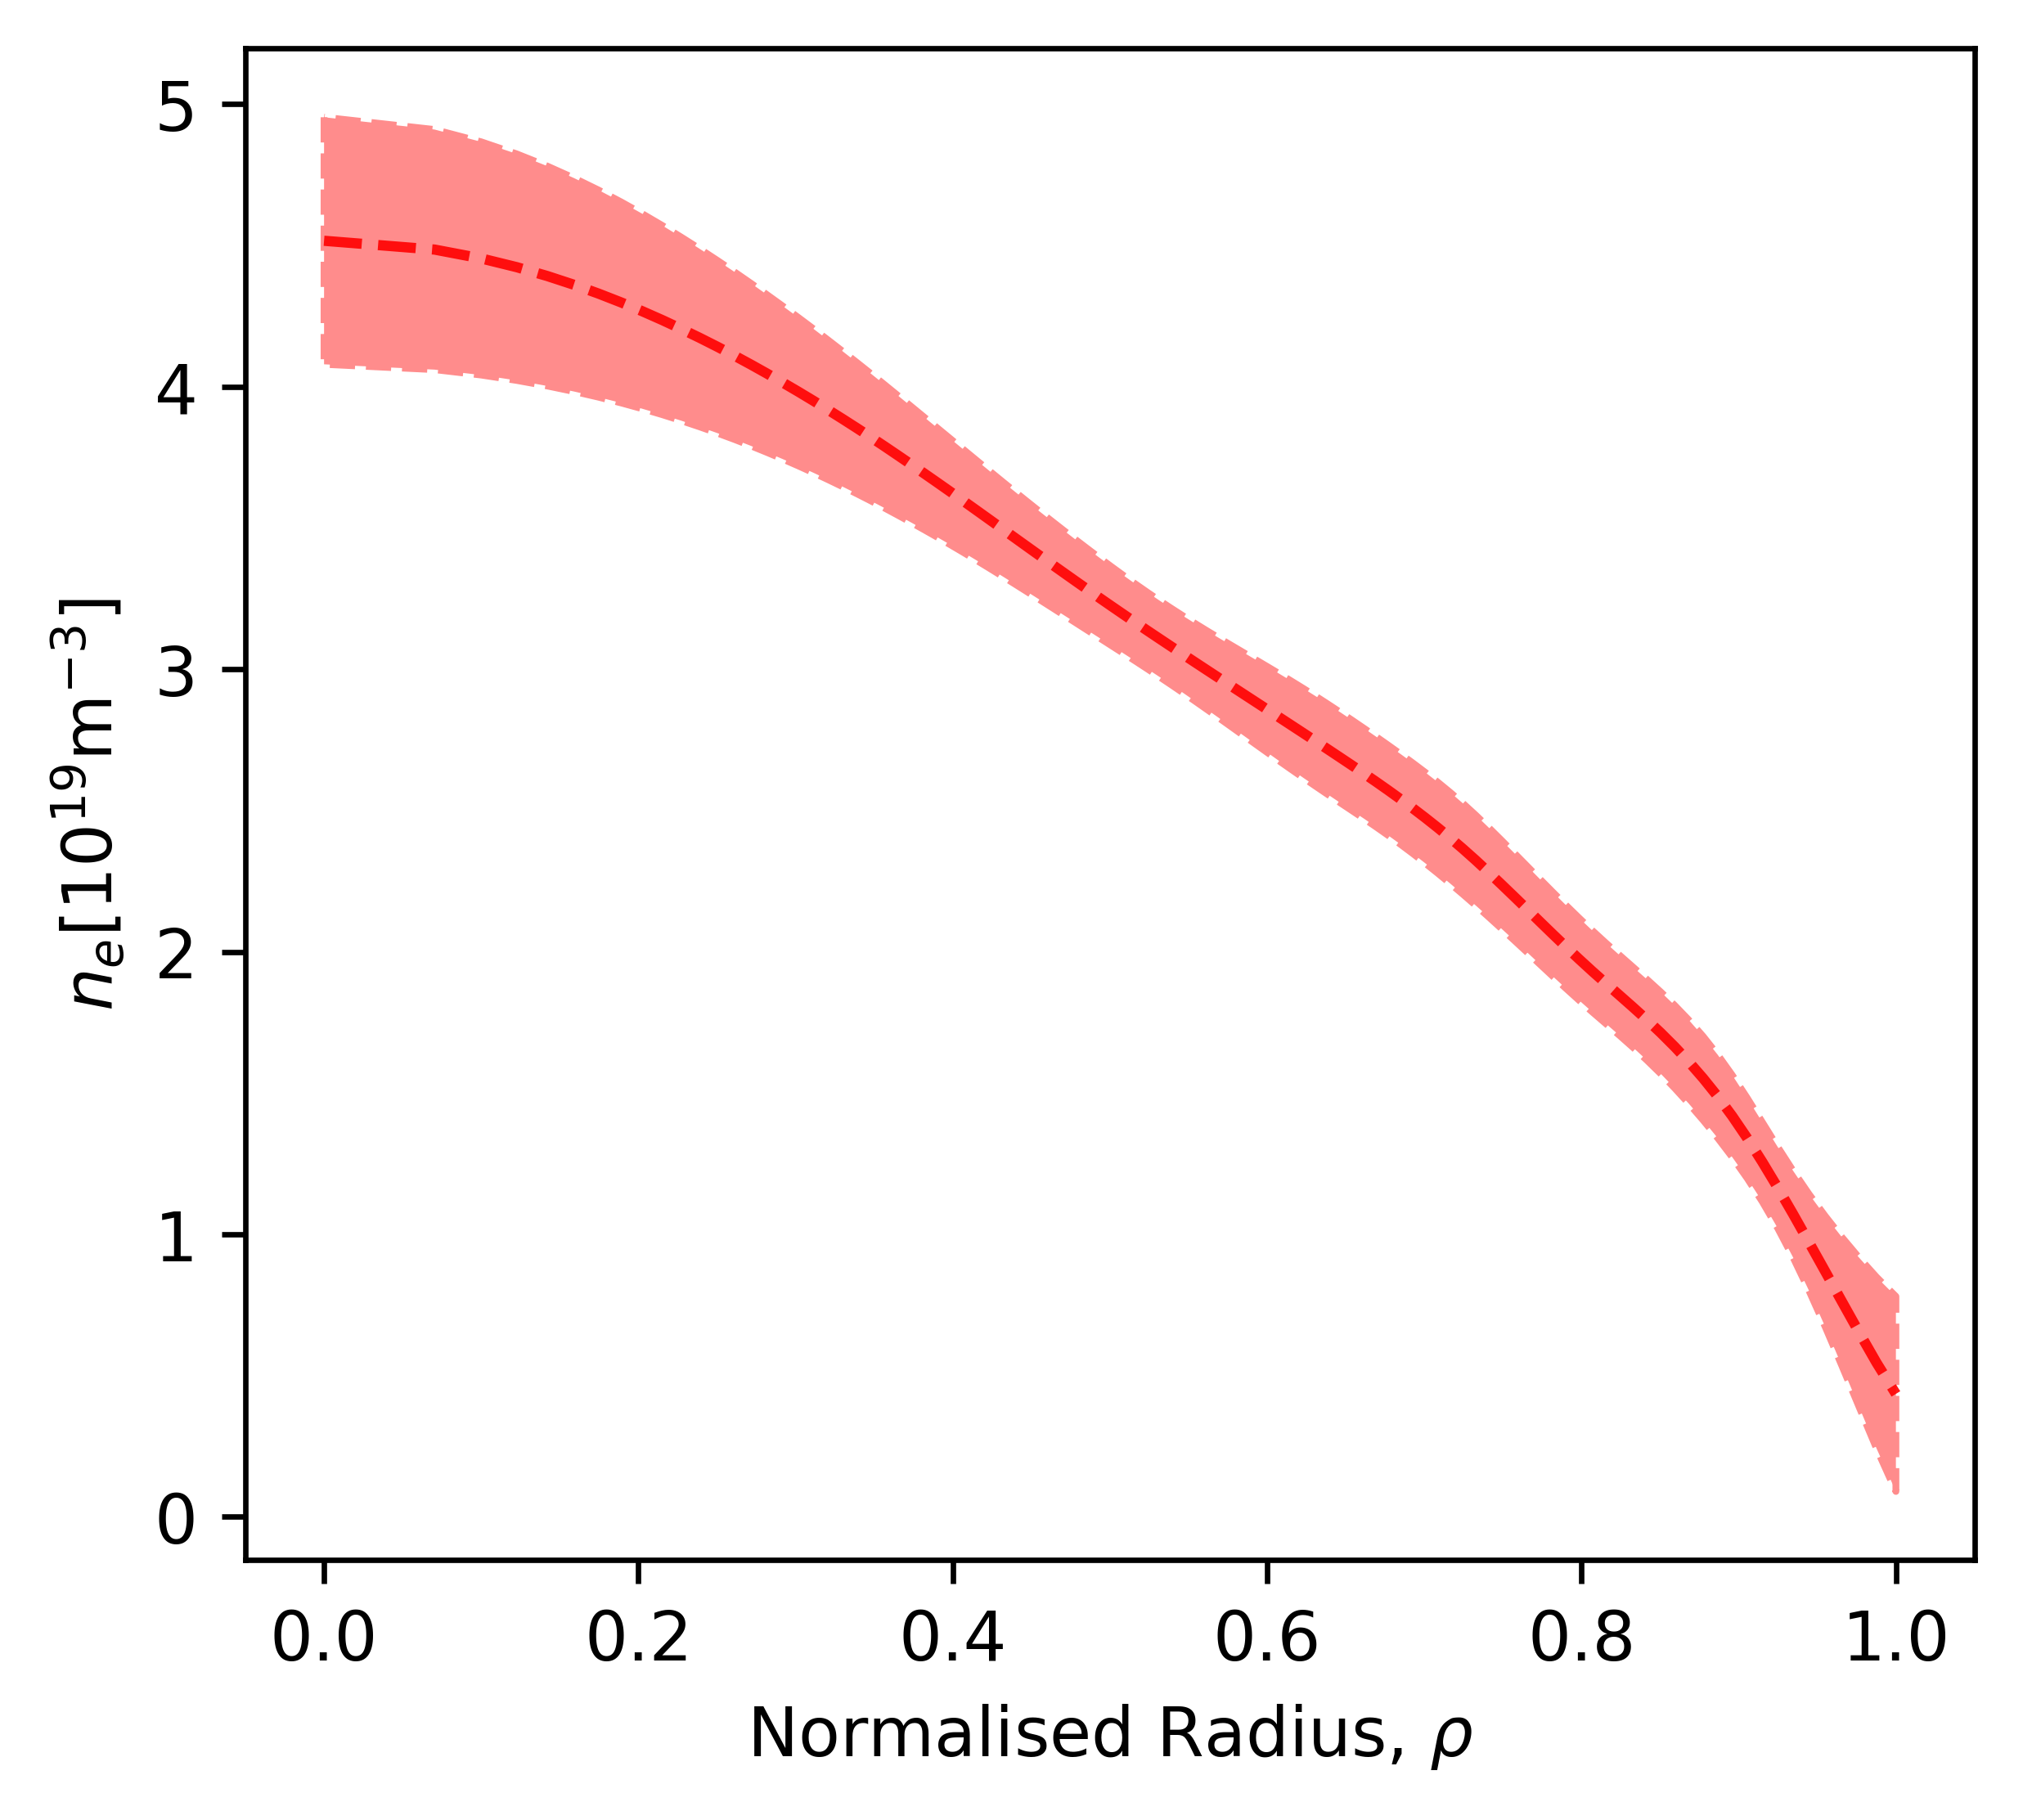
\includegraphics[width=\columnwidth]{images/niceExample.png}
%   \hskip 1mm
%   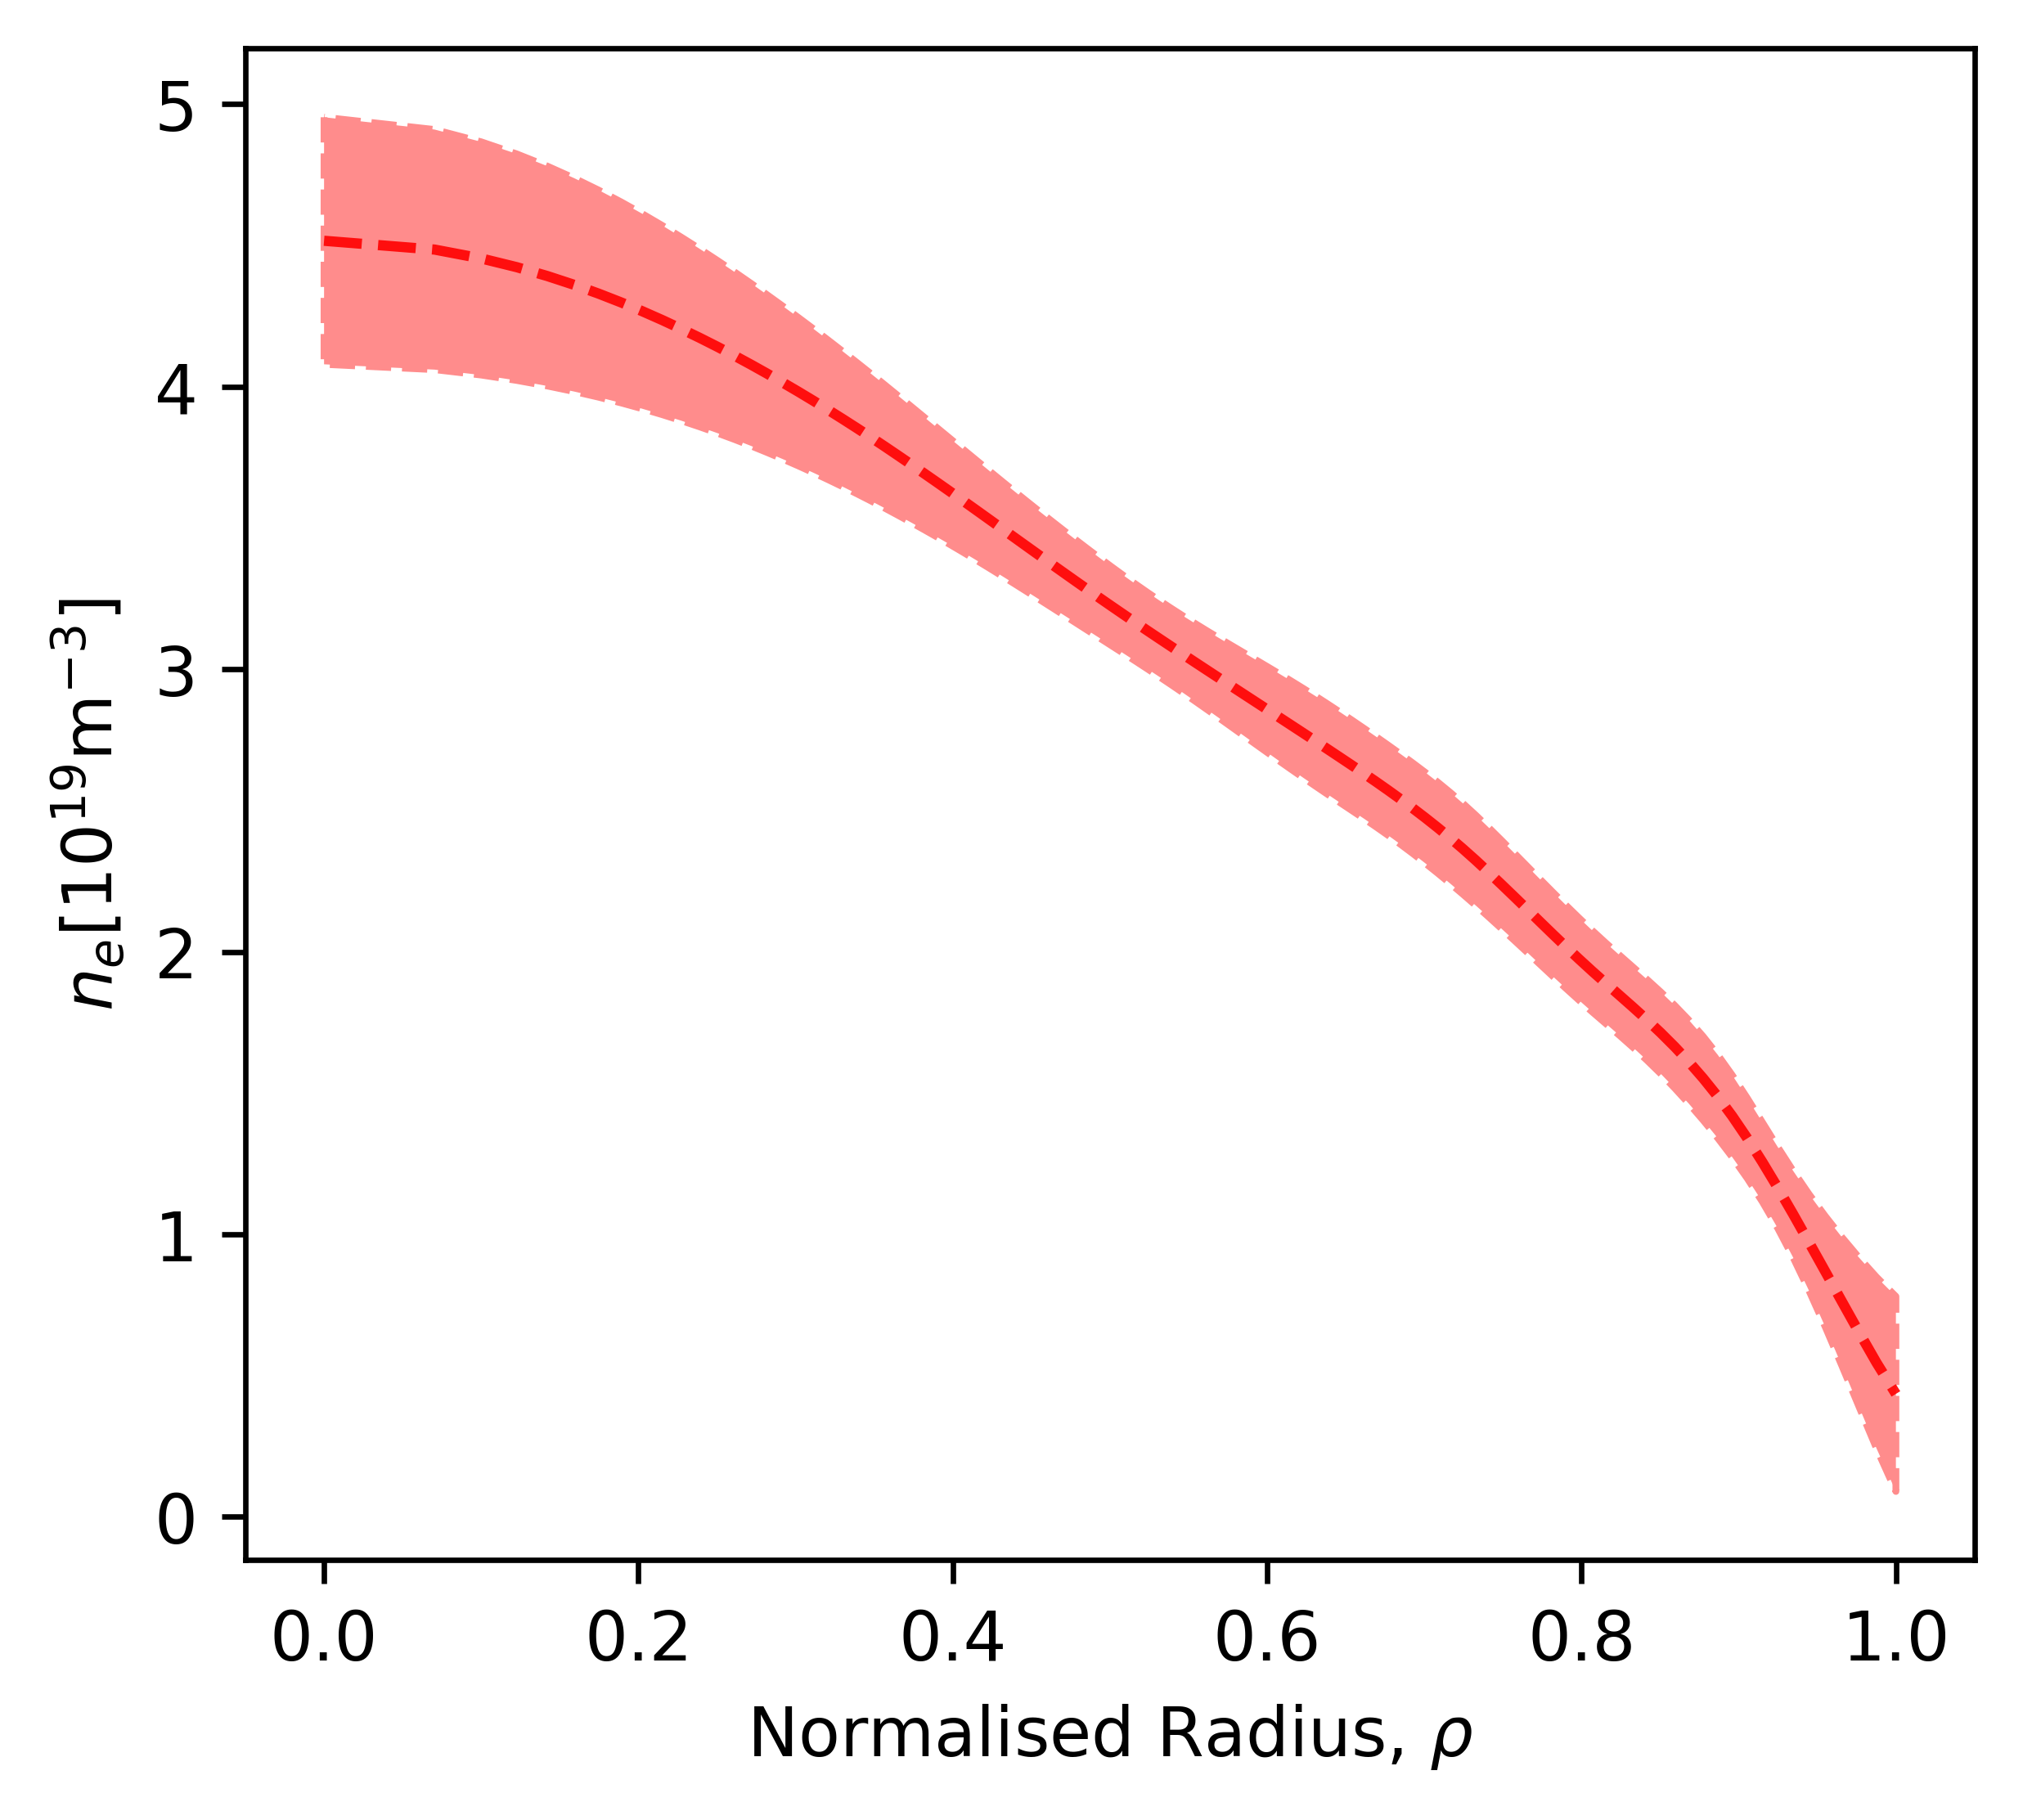
\includegraphics[width=\columnwidth]{images/niceExample.png}
%   \hskip 1mm
%   \vspace{-1cm}
%   \caption{Predictions on completely sampled space.}
%   \label{fig:flowe_grid}
% \end{figure}

% \label{sec:intpol}
% \section{Interfero-polarimetry}
\begin{itemize}
    \item Some basic backround theory of a tokamak as a fusion device. Including the schematics of the magnetics and different systems present. Including the magnetic flux surfaces and what they are, assumptions made. What is $\rho$? Also highlights a little why plasma density profile is important. 
    \item Explain the theory of how NICE did their inference to some degree. ***
    \item Bayes Theorem for inference problems, each distribution involved and why the margianl likelyhood is useful. ***
    \item Explian how a multivariate gaussian can model a curve. ***
    \item Explain Gaussian Process Regression for a generic line fitting problem, including the various distributions constructed and how they are used in the closed form expressions. A little on marginal liklyhood again for parameter optimisation. Mention briefly the alterations to this algorythem that will be made to allow it to be used for interferometry including the responce function change, and virtual observations.
    \item Explain Interferometry and a little on polarimetry, show west laser geometry
    \item Explain the magnetic flux surfaces again a little and how this allows us to make the electron density profile 1D again.
    \item Explain the forward model and how it is computed with the responce matrix.
    \item Explain how the prior edge and core information can be added and the complications of inserting it into the prior.
    \item Explain why a non stationary kernel (smooth step) might be beneficial 
    \item summarise the chapter and explain how it ties into the methodology
\end{itemize}





